\NeedsTeXFormat{LaTeX2e}
\documentclass[12pt,a4paper]{article}
\usepackage{german,a4}
\usepackage{epsfig}
\begin{document}

%%% TITLE =============================================================

\begin{titlepage}

\vspace*{\fill}
\begin{center}
\Huge{\bf{Ein Browser f\"{u}r Alice}}
\end{center}

\vspace{1cm}

\begin{center}
  \begin{minipage}[center]{10cm}
    \begin{tabbing} 
      \large{Bernadette Blum} \hspace{1cm}\= \large{Marvin Schiller}\\
      blum@ps.uni-sb.de \> schiller@ps.uni-sb.de\\[1cm]

      Betreuer: \\[2mm]
      \large{Thorsten Brunklaus} \> \large{Andreas Rossberg}\\
      brunklaus@ps.uni-sb.de \> rossberg@ps.uni-sb.de

    \end{tabbing}
  \end{minipage}
\end{center}

\vspace{5mm}
\begin{center}
\Large{6. Mai 2003}
\end{center}

\vspace{1cm}

\begin{center}
  \begin{minipage}[center]{5cm}
    Leitung:\\
    \large{Prof. Dr. Gert Smolka}\\
    smolka@ps.uni-sb.de
  \end{minipage}
\end{center}

\vspace{5mm}

\begin{center}
  \begin{minipage}[center]{5cm}
    Fachbereich Informatik\\
    Universit\"{a}t des Saarlandes\\
    Im Stadtwald \\
    66123 Saarbr\"{u}cken
  \end{minipage}
\end{center}

\vspace*{\fill}

\end{titlepage}

\begin{abstract}
Dieser Bericht zeigt Design und Implementierung eines 
interaktven Browser-Tools f\"{u}r die funktionale Programmiersprache 
Alice. Da Alice-Werte nicht selbstbeschreibend sind, 
mu\ss \, der Browser jeweils explizite Typinformationen zu denjenigen  
Werten erhalten, die dargestellt werden sollen. 
Um Werte abstrakter Typen in eine entsprechende Darstellung 
transformieren zu k\"{o}nnen, wird weiterhin 
deren Registrierung beim Browser erforderlich. 
Der Browser ist in Alice selbst implementiert und verwendet die Gtk-Bibliothek
zur Erzeugung der graphischen Benutzerschnittstele.
Unser Design kn\"{u}pft weitgehend an Thorsten Brunklaus' ''Oz Inspektor'' 
\cite{br:oz} an.
\end{abstract}


%%% EINFUEHRUNG ==========================================================

\section{Einf\"{u}hrung}  

\paragraph{}

Die graphische Aufbereitung von Programmen und Datenstrukturen erm\"{o}glicht 
Programmierern das Debuggen komplexer Programme. 
Dazu werden Algorithmen entwickelt, die man als ``Pretty Printer'' bezeichnet. 
Ziel bei der Entwicklung von Pretty Printern ist es, die Lesbarkeit eines 
Dokuments (meist Programme und mathematische Ausdr\"{u}cke) durch 
Einr\"{u}ckungen, gezielte Zeilenumbr\"{u}che und 
visuelle Atribute zu verbessern.
Dieser Bericht stellt Design und Implementierung 
eines solchen ``Pretty Printers'' f\"{u}r die Programmiersprache Alice vor. 

\paragraph{}

Die funktionale Programmiersprache Alice erm\"{o}glicht nebenl\"{a}ufige 
Programmierung und die Erzeugung zyklischer Datenstrukturen. 
Dies erlaubt es dem Programmierer, Berechnungsstr\"{a}nge (sog. Threads) 
willk\"{u}rlich zu starten oder zu beenden, Werte erst bei 
Bedarf auswerten zu lassen (sog. Laziness), oder Platzhalter 
f\"{u}r noch nicht bekannte Berechnungsergebnisse einzusetzen (sog. Futures).
\\
Die daraus resultierende Komplexit\"{a}t erfordert eine Darstellung, 
die diesen Konzepten in \"{U}bersichtlichkeit und Flexibilit\"{a}t gerecht 
wird.

\paragraph{}

Anders als beispielsweise in der Programmiersprache Oz sind 
Typen in Alice nicht selbstbeschreibend. Dadurch mu\ss \, 
zur graphischen Darstellung eines Alice-Wertes durch den 
Browser nicht nur 
der Wert selbst, sondern auch strukturelle 
Information zu diesem Wert \"{u}bergeben werden. Diese l\"{a}sst sich durch 
sogenannte Typreflektion gewinnen. Dieser Bericht zeigt auf, 
wie der Browser die strukturelle Information 
bei der Darstellung der dazugeh\"{o}rigen Werte gesteuert wird und 
welche Mechanismen n\"{o}tig sind, um Werte beliebiger abstrakter Typen 
darstellen zu k\"{o}nnen.


%%% ZENTRALE IDEEN =====================================================

\section{Zentrale Ideen}

Der Browser soll in der Lage sein, Alice-Werte 
\"ubersichtlich auf einem graphischen Interface darzustellen. 
Dies wird erreicht, indem die Werte in eine interne Beschreibung 
transformiert werden, aus der die graphische Repr\"asentation 
erzeugt werden kann. 
Dies wird in Abbildung 2.1 verdeutlicht. 
Die Transformation in 
die interne Beschreibung wird durch die 
Typinformation der inspizierten Werte gesteuert. 

\begin{center}
\begin{picture}(360,470)
\put(0,370){\framebox(360,100){\begin{math}
                                \begin{array}{clcr}
                                  (
                                  \{
                                   eins $=$ \sharp ''1'' ,
                                  zwei $=$ \sharp ''2'' \} , 
                                  \{ drei $=$  3 , 
                                  vier $=$  4 \} ) \\ 
                                  \bf{+}   \\
                                   Typreflektion 
                                  ( \{eins: char, zwei: char\},
                                  \{drei: int, vier: int\} )
                                \end{array}  
                                \end{math}}}
\put(180,360){\vector(0,-4){30}}
\put(80,220){\framebox(200,100){Browser-interne Wertbeschreibung}}
\put(180,210){\vector(0,-4){30}}
\put(40,0){
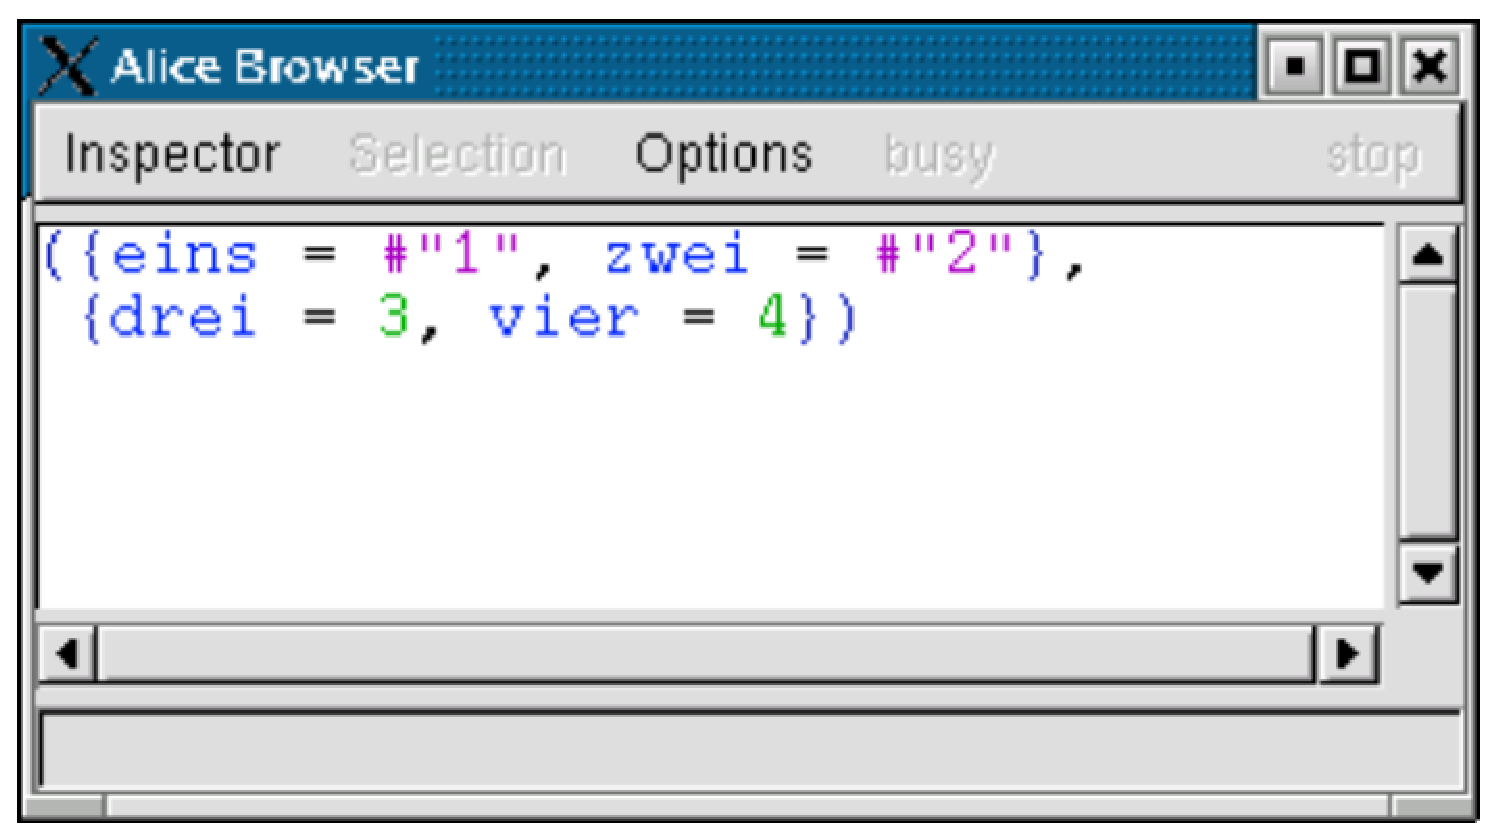
\epsfig{file = 3stepsgui.ps, width=10cm}}
\end{picture}
\newline
\nopagebreak
Abbildung 2.1: Zusammenhang zwischen Wert- und Typinformation, interner 
Wertbeschreibung und Darstellung auf der GUI
\end{center}

\subsection{Typregistrierung}

\paragraph{}

Die Typen von Alice-Werten k\"onnen strukturelle oder abstrakte Typen 
sein. Um die Werte in eine entsprechende Darstellung transformieren 
zu k\"onnen, ben\"otigt der Browser explizite strukturelle  
Information zu diesen Werten. 

\paragraph{}

Gleichzeitig ben\"otigt der Browser Anweisungen, wie 
ein Wert eines bestimmten Types in eine interne 
Repr\"asentation und letztendlich eine graphische Darstellung 
umgewandelt werden soll.

\paragraph{}

W\"ahrend strukturelle Typen die ben\"otigte Strukturinformation 
zu dieser Transformation liefern, m\"ussen abstrakte Typen 
zusammen mit Darstellungsanweisungen beim Browser registriert 
werden. Diese Darstellungsvorschriften werden in Form einer 
Prozedur \"ubermittelt, welche die Umwandlung in eine 
Beschreibung des Wertes spezifiziert.  

\subsection{Darstellungskriterien}

\paragraph{}

Der Entwurf eines graphischen Tools erfordert die \"Uberlegung, 
welche Kriterien bei der Wahl von Anordnungsvorschriften f\"ur 
die Darstellung der Datenstrukturen im Vordergrund stehen sollen. 
Es gibt Pretty Printer, die, wie auch der 
Algorithmus von Oppen \cite{op:pr}, die Einhaltung einer vorgegebenen 
darstellbaren Seitenbreite sicherstellen, und durch gezielte 
Umbr\"uche und Einr\"uckungen die Lesbarkeit wiederherstellen. Im 
Gegensatz dazu steht die Vorgehensweise, die Anordnung nicht 
an einer vorgegebenen Seitenbreite zu orientieren, sondern 
vielmehr die Gr\"o\ss e des Darstellungsbrereichs an eine m\"oglichst 
\"ubersichtliche Darstellung anzupassen. 
Im Fall des Alice-Browsers wurde letztere Vorgehensweise gew\"ahlt, 
um trotz der Komplexit\"at der Alice-Datenstrukturen 
eine klare Darstellung zu erm\"oglichen.

\paragraph{}

Zusammengesetzte Alice-Werte lassen sich in Teilwerte untergliedern, 
so dass sich ein solcher Wert 
in eine baumartige Darstellung zerlegen l\"asst.
Hier deutet sich schon an, 
dass sich auch die interne Behandlung der Datenstrukturen 
an Baumstrukturen orientieren muss. Gleichzeitig soll der Browser 
bei der graphischen Darstellung auf 
die f\"ur Alice \"ubliche Notation f\"ur 
Werte mit Klammern und Trennzeichen 
zur\"uck greifen.    
Die Darstellung von baumartigen Werten durch 
den Browser orientiert sich dabei 
an einer Regel, wie sie u.a. Kennedy \cite{ke:dr} f\"ur 
das Baumzeichnen aufstellt: Gleiche Teilb\"aume werden 
gleich dargestellt. 





%%% ENTWURF ============================================================

\section{Entwurf}

%%% Bild: create -> layout -> draw

\subsection{Interne Darstellung}

\subsection{Typregistrierung}

\subsection{Transientenverwaltung}

\subsection{Graphmodus}

\subsection{Filter} 


%%% IMPLEMENTIERUNG ====================================================

\section{Implementierung}

\subsection{Knotentypen}

\subsection{Typregistrierung und -zerlegung}

\subsection{Layout}

\subsection{Zeichnen}

\subsection{Transientenverwaltung}

\subsection{Inkrementalit\"at}

Die Darstellung der inspizierten Alice-Werte auf 
der graphischen Benutzeroberfl\"ache mu\ss \, 
schnell an Ver\"anderungen der inspizierten 
Werte angepasst werden k\"onnen. Dies 
wird unter anderem dann erforderlich, wenn 
eine Wertzuweisung an einen Transienten 
erfolgt, so da\ss \, die Darstellung des 
neuen Wertes die Darstellung des Transienten 
auf der Benutzeroberl\"ache ersetzen soll. 
Diese Ver\"anderungen erfolgen inkrementell, 
d.h. ausgehend von der bereits bestehenden 
Darstellung wird m\"oglichst wenig Berechnungsaufwand 
getrieben, um zur neuen Darstellung zu gelangen.

\begin{center}
\epsfig{file = incr1.ps, width = 10cm}
\newline
\end{center}
Abbildung ? \\[1cm]


Abbildung ? stellt die interne 
(baumartige) Beschreibung einer Datenstruktur 
dar. Es wird angenommen, da\ss \, die Darstellung 
des markierten Teilbaums ersetzt werden mu\ss .

\begin{center}
\epsfig{file = inkr2.ps, width = 10cm}
\newline
\end{center}
Abbildung ? \\[1cm]


Abbildung ? zeigt die n\"otigen Schritte, um zu einer 
neuen Beschreibung und zu einer neuen Darstellung 
auf der Benutzeroberfl\"ache zu gelangen. 
Der betroffene Teilbaum selbst mu\ss vollkommen neu konstruiert, 
angeordnet und dessen graphische Repr'\"asentation 
gezeichnet werden. Da dies die Anordnung des 
gesamten Knoten st\"{o}ren kann, mu\ss \, auf dem Pfad von 
diesem Teilbaum zum 
Wurzelknoten die Anordnung neu berechnet werden. Dies kann 
zur Folge haben, da\ss  von der \"{A}nderung nicht direkt 
betroffene Teilb\"{a}ume an neue Positionen verschoben 
werden m\"{u}ssen. 

Von diesen Positions\"{a}nderungen 
abgesehen k\"{o}nnen diese Teilb\"{a}ume unver\"{a}ndert 
beibehalten werden. Dies ist g\"{u}nstiger, als den gesamten 
Baum neu zu konstruieren, anzuordnen und zu zeichnen.   
 

\subsection{Module}

\begin{center}
\epsfig{file = module_bw.ps, width = 13cm}
\linebreak Abbildung 4.6: Module des Browsers
\end{center}

Abbildung 4.6 zeigt die Module des Browsers.
Dieser verf\"{u}gt \"{u}ber zwei Module, die 
die Datentypen der internen Beschreibung  - doc und node - enthalten. 
Neben den Datentypen beinhalten die Module \"{u}ber 
entsprechende Accessoren.
Da diese w\"{a}hrend der 
Erzeugnung, der Anordnungsberechnung, dem Zeichnen 
und der Darstellungsab\"{a}nderung verwendet werden, 
werden diese Module in vielen anderen Modulen benutzt.\\
Das Modul GtkSupport kapselt die Gtk-Funktionalit\"{a}t 
gegen\"{u}ber allen anderen Modulen des Browsers ab. 
Als einziges Modul hat es direkten Zugriff auf die 
Gtk-Prozeduren. Die anderen Module des Browsers 
greifen dabei auf GtkSupport zur\"{u}ck.
Die Module CreateTree, Layout, und Draw repr\"{a}sentieren 
die drei Phasen des Inspektionsvorgangs, w\"ahrend das Modul 
Update die notwendigen Mechanismen repr\"asentiert, 
um die Darstellung an Ver\"{a}nderungen anzupassen. 
Das Modul Widget verf\"{u}gt \"{u}ber die 
graphische Benutzeroberfl\"{a}che und steuert 
die Darstellungserzeugung bzw. Ver\"{a}nderung. 
Letztendlich macht das Modul UnsafeInspector die f\"{u}r den 
Benutzer relevanten Prozeduren und Datentypen nach au\ss en sichtbar.



%%% AUSBLICK ===========================================================

\section{Ausblick}

Zur Zeit verwenden wir ein Gtk-Binding f\"ur Mozart \cite{mo:mo}
zur Erzeugung der graphischen Benutzeroberfl\"ache. Allerdings ist 
es auch m\"oglich, den Browser an eine von Robert Grabowski im Rahmen 
seines Fortgeschrittenenpraktikums neu implementierte Gtk-Schnittstelle
f\"ur Alice \cite{gr:gt} anzuschlie\ss en.

\paragraph{}

Desweiteren ist der Alice-Browser nicht typsicher, 
da der Benutzer zur Zeit ein Tupel aus 
Wert und mithilfe des Typreflektors reflektierten Typs 
an die inspect-Funktion \"ubergibt.  
Eine automatische Typreflektion w\"urde die Benutzung des Tools 
erleichtern und eine Fehlbenutzung ausschlie\ss en. 
In diesem Fall m\"usste der Benutzer nur noch den zu 
inspizierenden Wert \"ubergeben. 

Mithilfe eines \"ubergeordneten Funktors lie\ss e 
sich der Browser einkapseln.

%%% BIBLIOGRAPHIE =======================================================

\begin{thebibliography}{99}

\bibitem{br:oz} Thorsten Brunklaus 2000. {\em Der Oz Inspector - Browsen: 
    Interaktiver, einfacher, effizienter} Diplomarbeit, Universit\"{a}t 
    des Saarlandes, Fachbereich Informatik.
\bibitem{op:pr} Derek Oppen 1980.{\em Prettyprinting} ACM Transactions 
  on Programming Languages and Systems, Bd. 2, Nr.4, 1980, pp 465-483.
\bibitem{ke:dr} Andrew Kennedy 1996. {\em Drawing Trees} 
                Journal of Functional Programming, Bd. 6(3), pp. 527-534.
\bibitem{al:al} Alice-Homepage: www.ps.uni-sb.de/alice/
\bibitem{gt:gt} GTK+: The Gimp Toolkit: www.gtk.org 
\bibitem{mo:mo} The Mozart Programming System: www.mozart-oz.org/
\bibitem{gr:gt} Robert Grabowski 2003. {\em Eine Gtk-Schnittstelle f\"ur 
                Alice} 
                FoPra-Ausarbeitung, Lehrstuhl Prof. G. Smolka, 
                Universtit\"at des Saarlandes.

\end{thebibliography}

\end{document}

